% ======================================================================
% BLOQUE 4 — Mi trabajo de licenciatura
% ======================================================================
\section{Mi tesis}
\bloque{MI TESIS · UMD}

% ---------------------------------------------------------------- 34
\begin{frame}{¿Se ve la asimetría con muones puros?}
  \begin{columns}[c,onlytextwidth]
    \column{0.46\textwidth}
      \centering
      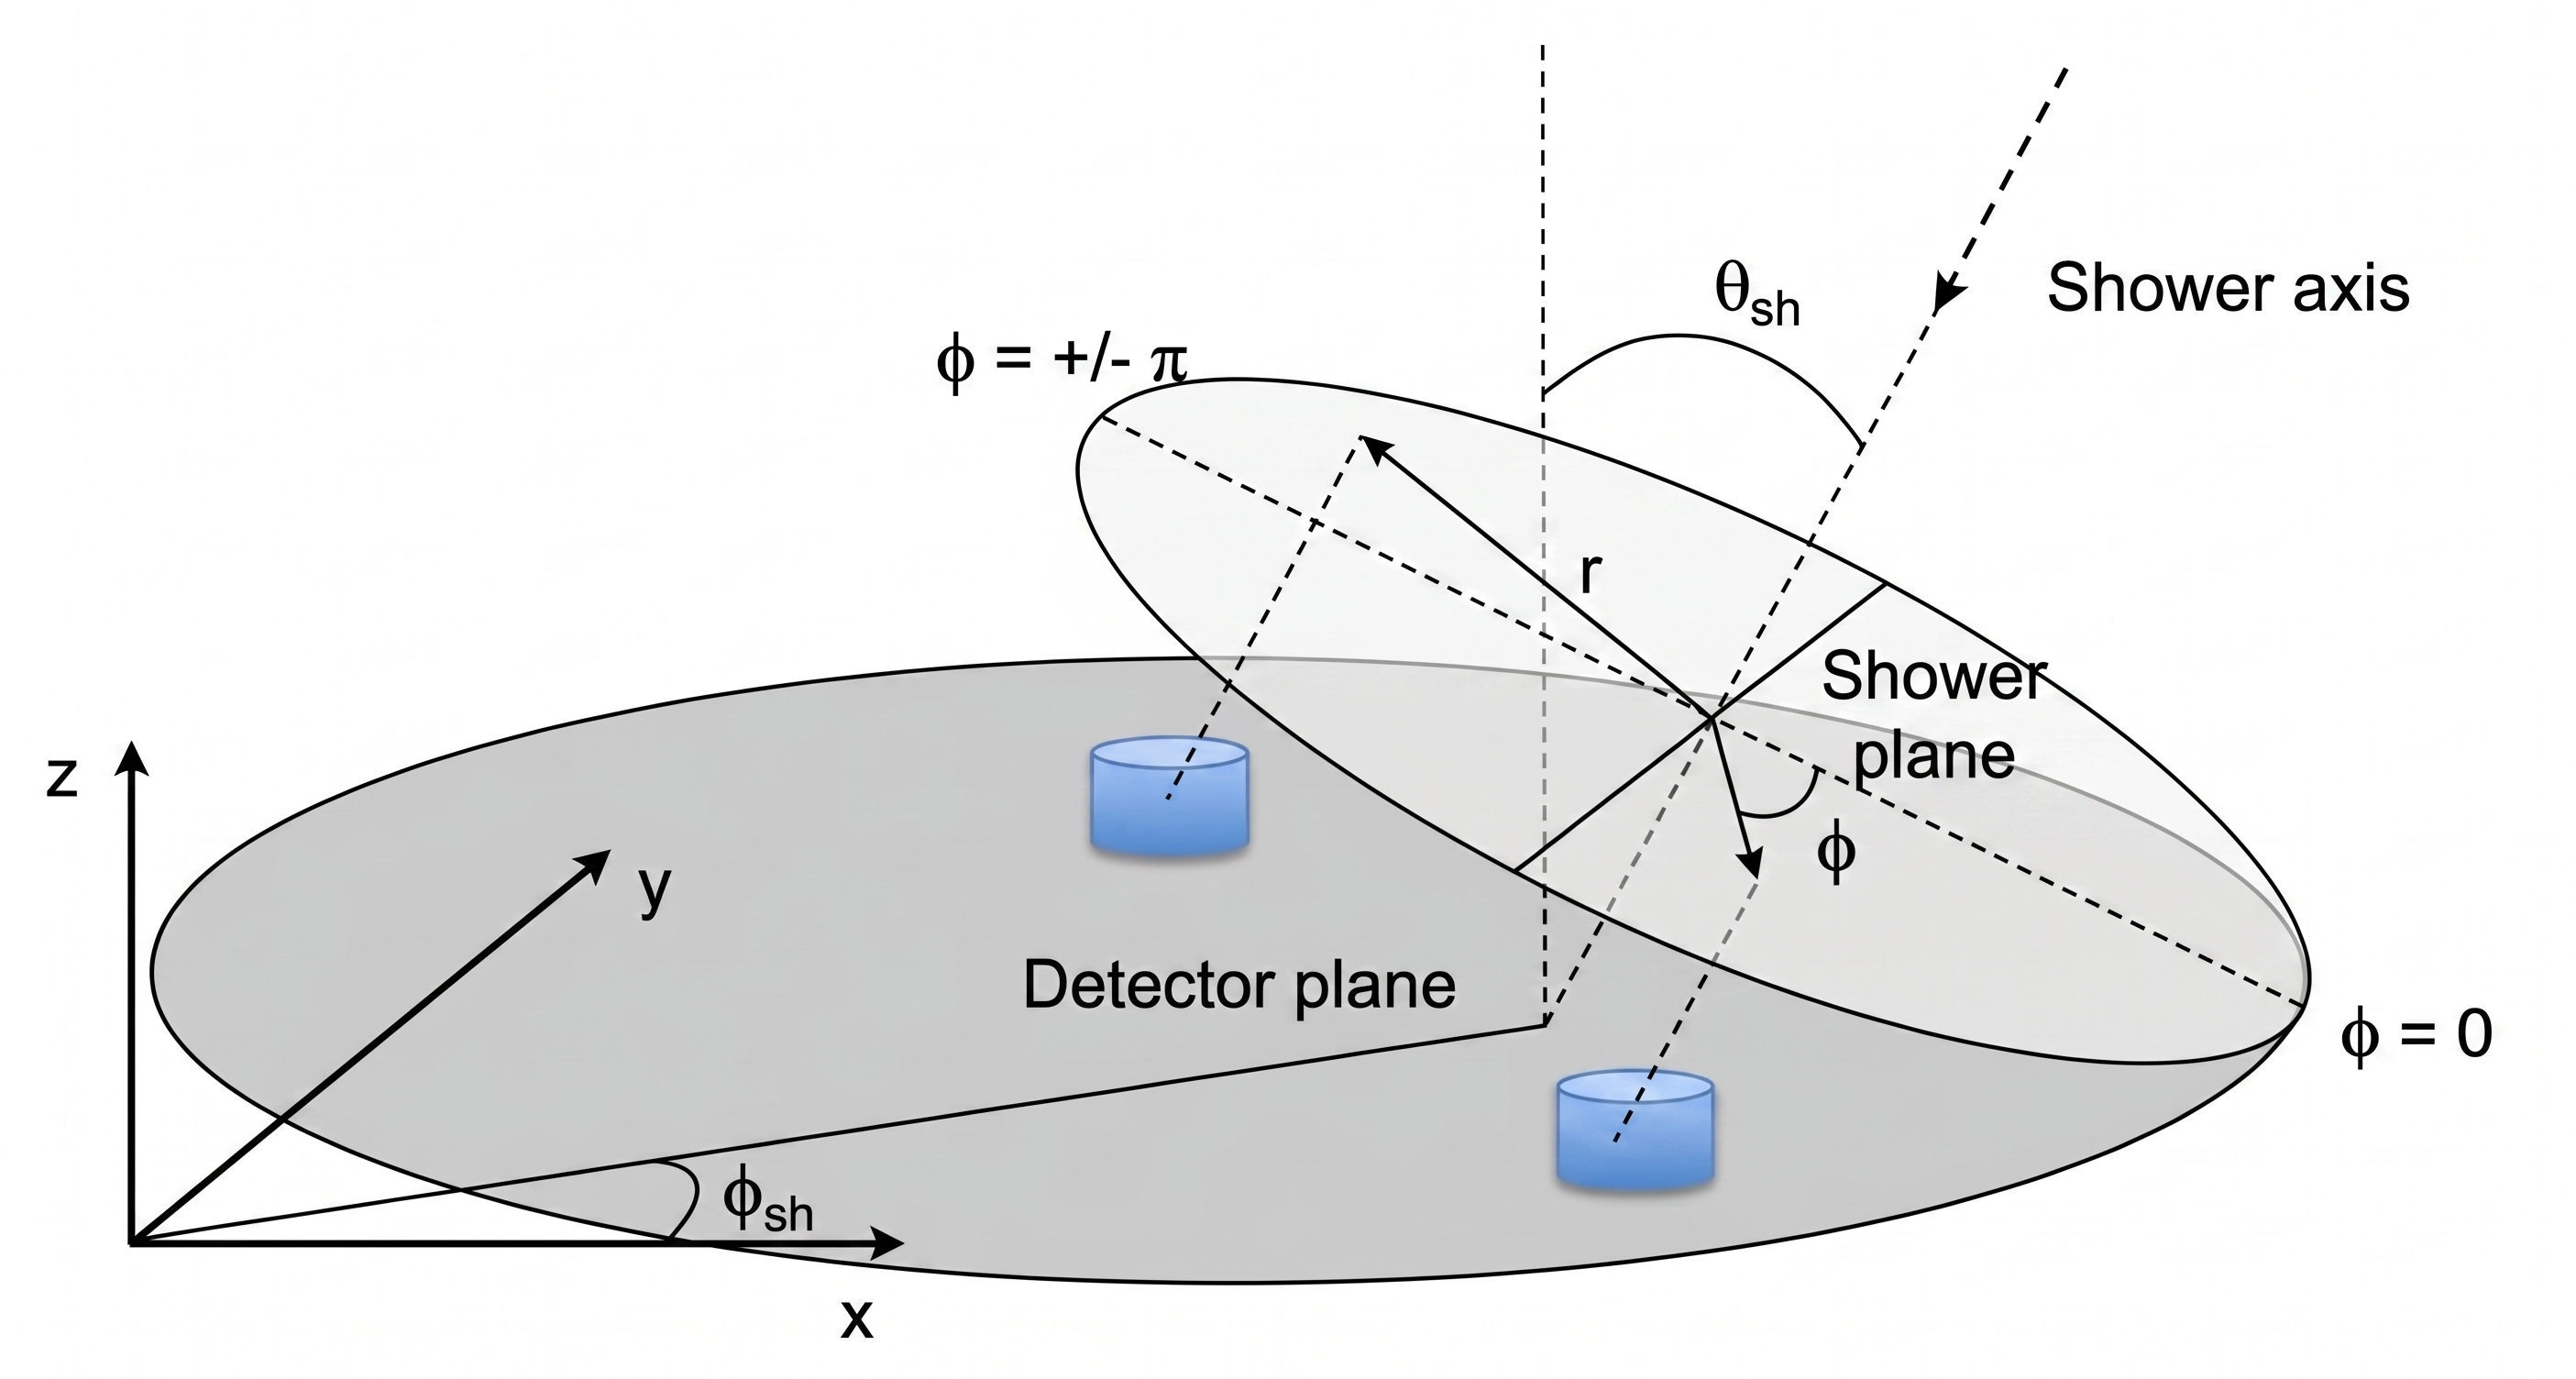
\includegraphics[width=0.92\linewidth]{tesis/esquema_lluvia.jpeg}\\[2pt]
      {\footnotesize Plano de la lluvia: $\phi=0$ es la región
      \textbf{temprana}, $\phi=\pm180^\circ$ la \textbf{tardía}.}
    \column{0.51\textwidth}
      \small
      En una lluvia inclinada la densidad en el suelo deja de ser circular:
      \[ \rho(\phi)=\rho_0\,\big(1+A_1\cos\phi\big) \]
      \begin{itemize}\footnotesize
        \item En el SD, $A_1$ de la señal \textbf{total} correlaciona con
          $X_\mathrm{max}$, pero mezcla electrones y muones.
        \item \textbf{Nunca se había estudiado con muones aislados}.
      \end{itemize}
      \vspace{-2pt}
      \begin{clave}
        \textbf{Objetivo}: caracterizar $A_1(r,\theta,E,A)$ en el UMD.
      \end{clave}
  \end{columns}
  \credito{Esquema: tesis de licenciatura (Silva Pizzi, FCEN-UBA, 2026), Cap.~3}
\end{frame}

% ---------------------------------------------------------------- 35
\begin{frame}{Cómo lo estudié}
  \begin{columns}[c,onlytextwidth]
    \column{0.50\textwidth}
      \begin{tikzpicture}[x=1cm,y=1cm,
        paso/.style={rounded corners=2pt, fill=itedaTeal, text=white,
          font=\scriptsize\bfseries, minimum height=0.62cm, inner sep=3pt, align=center},
        nota/.style={font=\tiny, text=itedaTealDark, align=left, anchor=west}]
        \node[paso] (a) at (0,3.0) {CORSIKA};
        \node[paso] (b) at (0,1.9) {Offline};
        \node[paso] (c) at (0,0.8) {Python};
        \node[paso, fill=itedaOrange] (d) at (0,-0.3) {ajuste de $A_1$};
        \draw[flecha, itedaGray] (a) -- (b); \draw[flecha, itedaGray] (b) -- (c);
        \draw[flecha, itedaGray] (c) -- (d);
        \node[nota] at (0.9,3.0) {lluvias de $p$, He, O, Fe; $10^{17{,}5}$--$10^{18}$\,eV;\\
          SIBYLL 2.3e, QGSJET-III.01, EPOS-LHC-R};
        \node[nota] at (0.9,1.9) {respuesta del SD y del UMD;\\reconstrucción como en los datos};
        \node[nota] at (0.9,0.8) {densidad de muones por módulo,\\en bines de $(r,\theta)$};
        \node[nota] at (1.25,-0.3) {primer armónico, errores \emph{bootstrap}};
      \end{tikzpicture}\\[6pt]
      \footnotesize
      \textbf{Dos geometrías de detector}: el \textbf{Anillo Denso} (12
      estaciones virtuales a 450\,m, cada 30$^\circ$) y el arreglo real de
      750\,m.\\[2pt]
      \textbf{Dos geometrías de lluvia}: la \textbf{verdadera} (MC) y la
      \textbf{reconstruida} (REC).
    \column{0.47\textwidth}
      \centering
      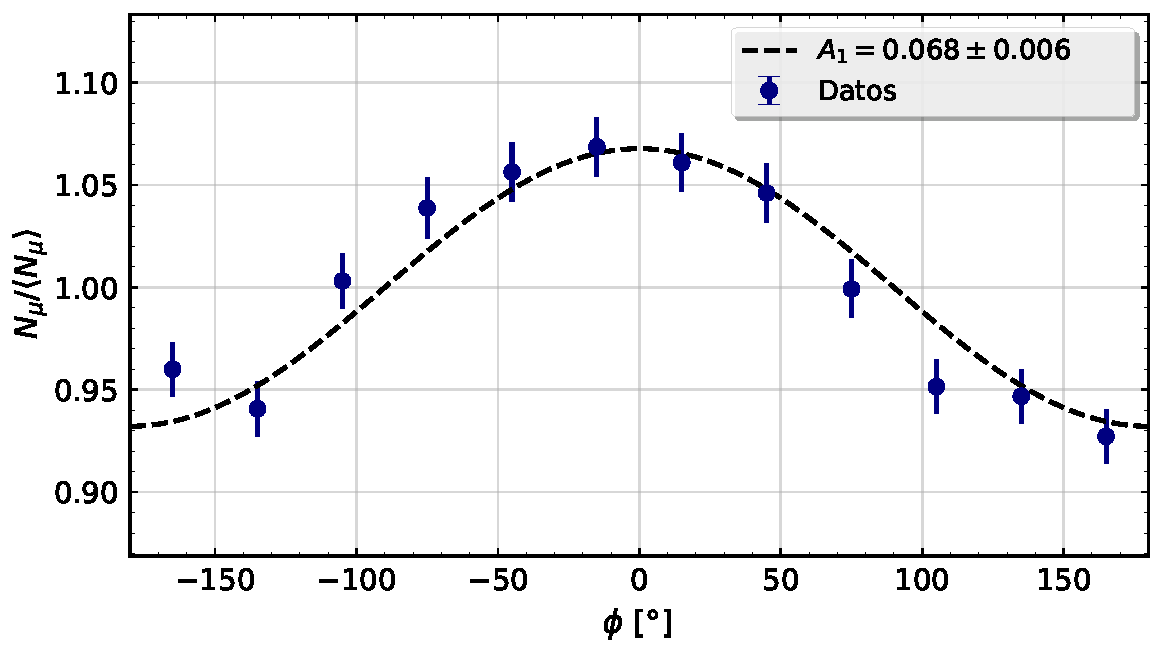
\includegraphics[width=\linewidth]{tesis/Ajuste_UMD_REC_Bin9.pdf}\\[1pt]
      {\footnotesize Anillo Denso, protones, $59^\circ$--$65^\circ$: la
      densidad de muones \textbf{reconstruida} sigue un coseno, con
      $\pm7\%$ entre regiones.}
  \end{columns}
  \credito{Figura: tesis, Cap.~5}
\end{frame}

% ---------------------------------------------------------------- 36
\begin{frame}{La asimetría sobrevive en los muones}
  \begin{columns}[T,onlytextwidth]
    \column{0.49\textwidth}
      \centering
      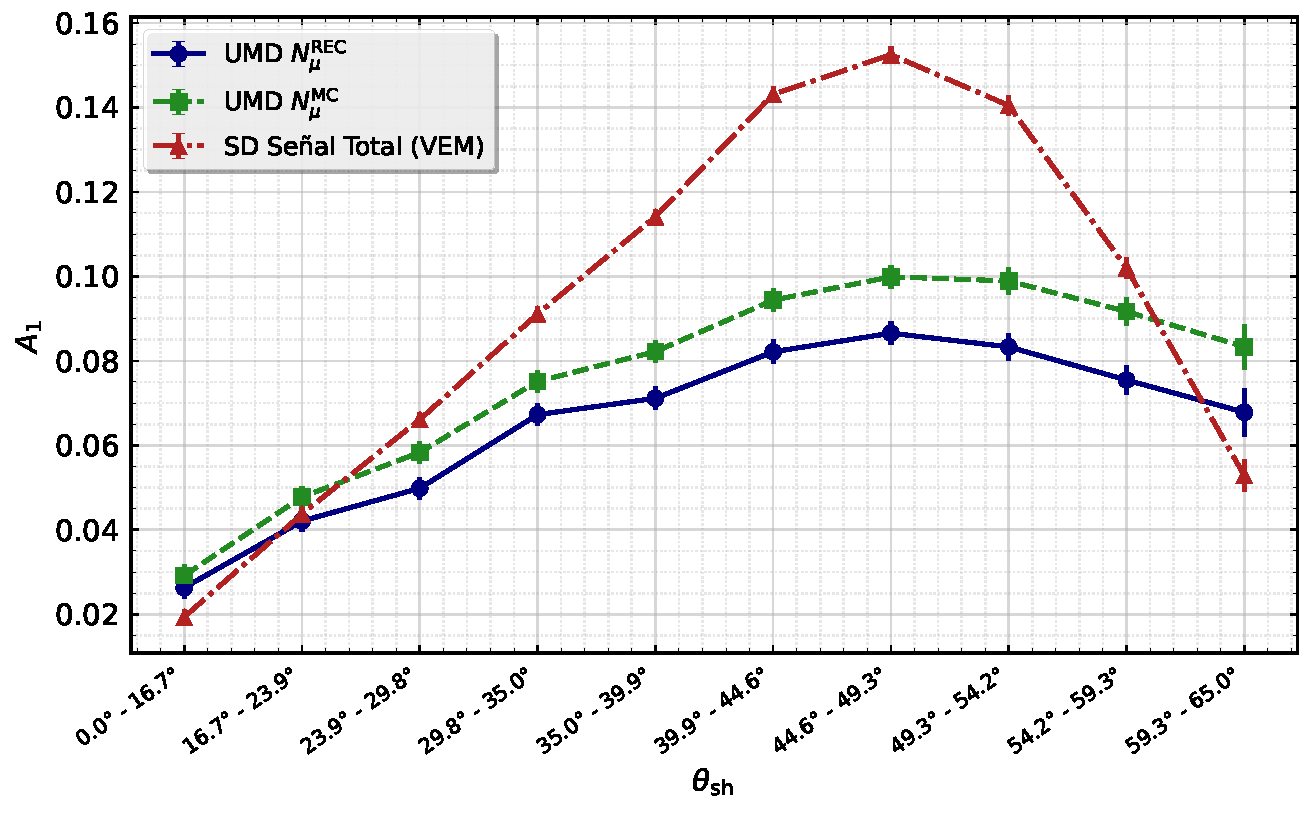
\includegraphics[width=0.88\linewidth]{tesis/Evolucion_Asimetria_vs_Theta.pdf}\\[1pt]
      {\footnotesize Crece con $\theta$: $A_1\approx0{,}09$ a 45--50$^\circ$,
      sin componente electromagnética.}
    \column{0.49\textwidth}
      \centering
      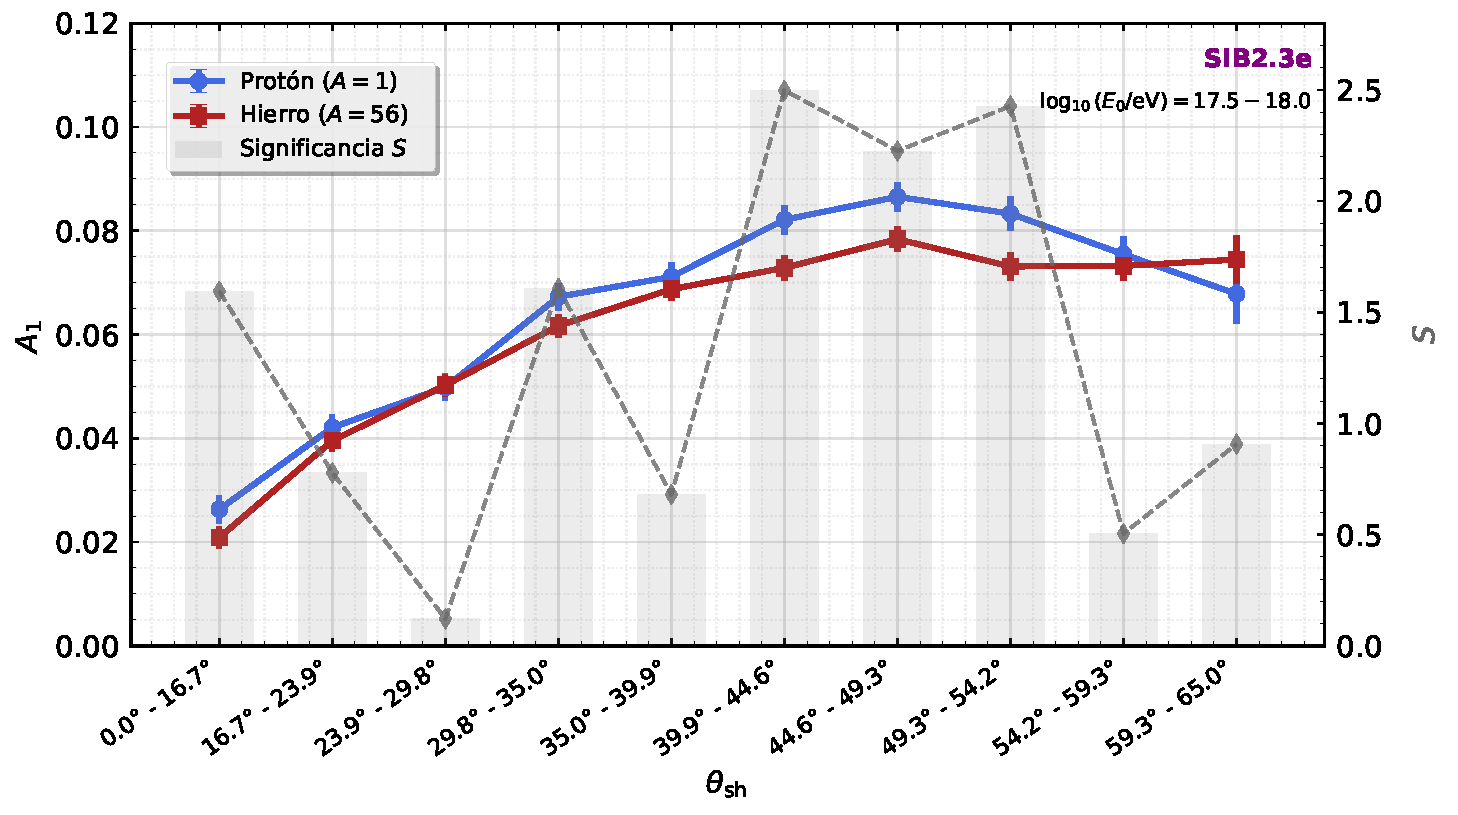
\includegraphics[width=0.88\linewidth]{tesis/Mass_Discrimination_MF.pdf}\\[1pt]
      {\footnotesize Protón por encima de hierro: diferencia de medias
      $\sim$2,5 veces su incerteza a 40--55$^\circ$.}
  \end{columns}
  \vspace{2pt}
  \begin{clave}
    $A_1\propto (r/D)\tan\theta$: un primario liviano acerca la producción
    de muones al suelo (menor $D$) y \textbf{aumenta} la modulación.
  \end{clave}
  \creditoizq{Figuras: tesis, Cap.~5 (Anillo Denso, SIBYLL 2.3e, $10^{17{,}5}$--$10^{18}$\,eV)}
\end{frame}

% ---------------------------------------------------------------- 37
\begin{frame}{Hallazgo 1: un sesgo de selección en el SD}
  \begin{columns}[c,onlytextwidth]
    \column{0.48\textwidth}
      \centering
      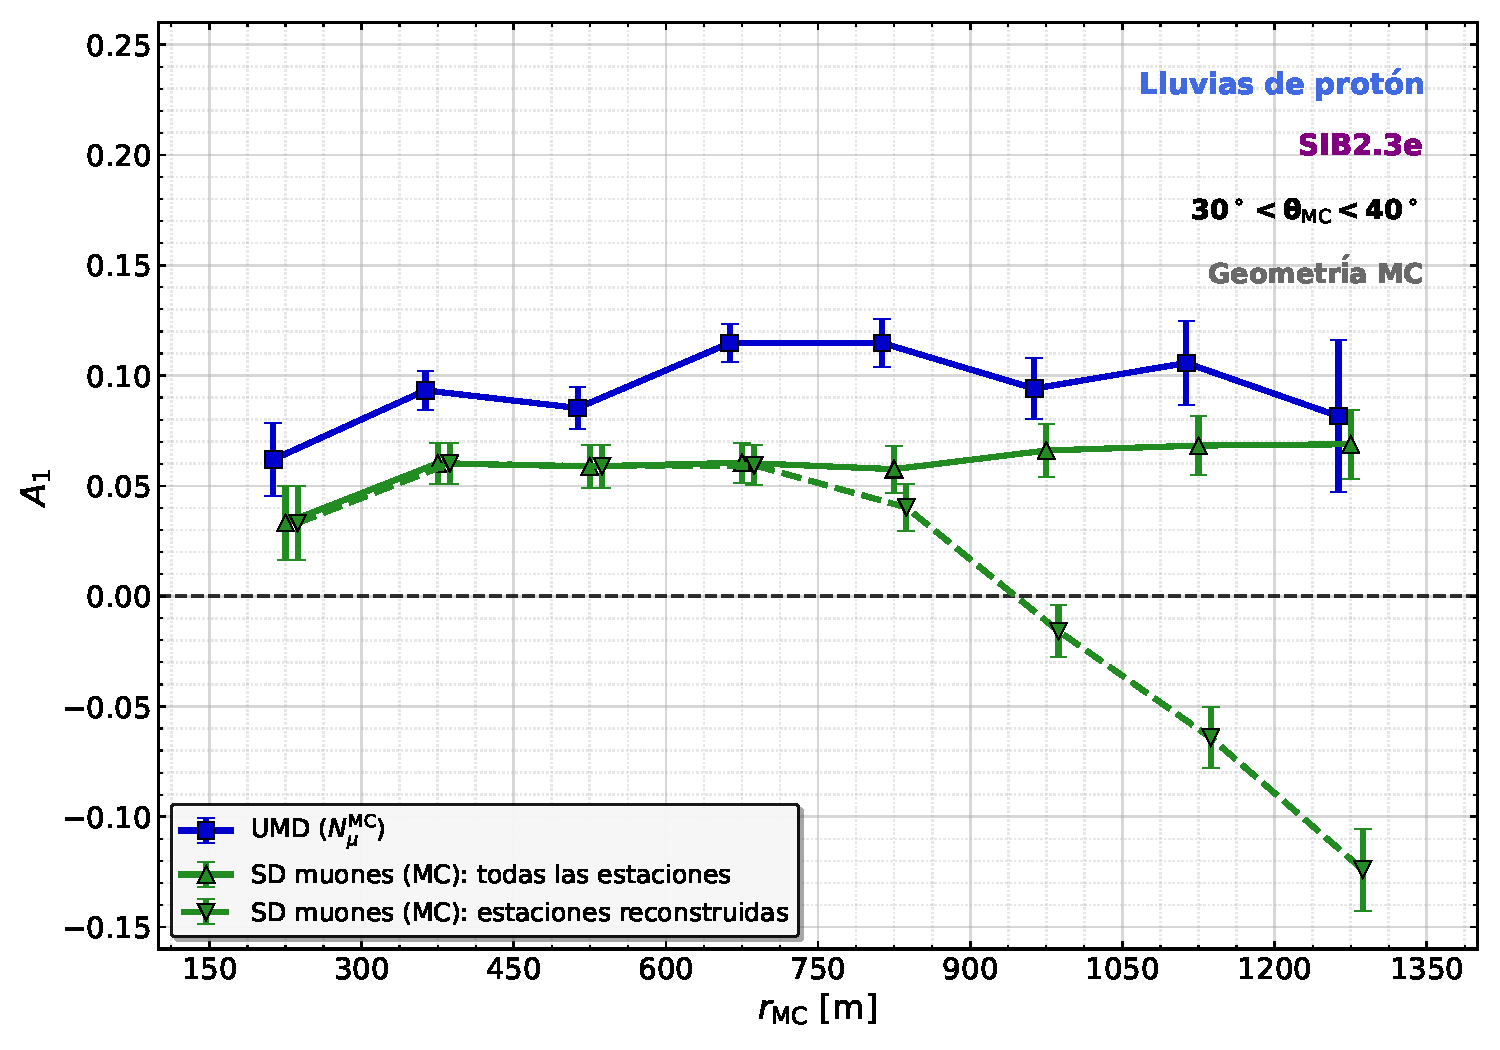
\includegraphics[width=\linewidth]{tesis/SD_Seleccion_Estaciones_vs_UMD.pdf}\\[1pt]
      {\footnotesize Mismos conteos de muones, mismo ajuste: sólo cambia
      \textbf{sobre qué estaciones se promedia}.}
    \column{0.49\textwidth}
      \centering
      \begin{tikzpicture}[x=1cm,y=1cm]
        \tikzset{
          tanque/.style={thick, fill=itedaLight, draw=itedaTeal},
          fuera/.style={thick, dashed, fill=white, draw=itedaGray!60},
          em/.style={fill=itedaOrange}, mu/.style={fill=itedaTealDark}}
        \node[font=\scriptsize\bfseries, text=cmbAzul] at (1.25,2.4) {región temprana};
        \node[font=\scriptsize\bfseries, text=cmbRojo] at (4.05,2.4) {región tardía};
        % temprana: las tres disparan (mucha señal EM); 0, 1 y 2 muones
        \foreach \x in {0,0.9,1.8}{
          \draw[tanque] (\x,0.9) rectangle ++(0.7,1.1);
          \foreach \k in {0.17,0.29,0.41,0.53}{\fill[em] (\x+\k,1.78) circle (1.2pt);}
          \node[font=\scriptsize, text=verdeRadio] at (\x+0.35,0.65) {\faCheck};}
        \fill[mu] (0.9+0.35,1.2) circle (2pt);
        \fill[mu] (1.8+0.22,1.2) circle (2pt); \fill[mu] (1.8+0.48,1.2) circle (2pt);
        % tardía: poca señal EM; sólo dispara la que tiene muones
        \draw[fuera] (2.8,0.9) rectangle ++(0.7,1.1);
        \draw[tanque] (3.7,0.9) rectangle ++(0.7,1.1);
        \draw[fuera] (4.6,0.9) rectangle ++(0.7,1.1);
        \foreach \x in {2.8,3.7,4.6}{\fill[em] (\x+0.35,1.78) circle (1.2pt);}
        \fill[mu] (3.7+0.22,1.2) circle (2pt); \fill[mu] (3.7+0.48,1.2) circle (2pt);
        \node[font=\scriptsize, text=cmbRojo] at (2.8+0.35,0.65) {\faTimes};
        \node[font=\scriptsize, text=verdeRadio] at (3.7+0.35,0.65) {\faCheck};
        \node[font=\scriptsize, text=cmbRojo] at (4.6+0.35,0.65) {\faTimes};
        \node[font=\tiny, anchor=west] at (0,0.2) {\textcolor{itedaOrange}{$\bullet$} $e^\pm,\gamma$
          \quad \textcolor{itedaTealDark}{$\bullet$} $\mu$ \quad
          \textcolor{verdeRadio}{\faCheck}\ forma parte del evento};
        \node[font=\scriptsize] at (1.25,-0.3) {$\langle N_\mu\rangle_\mathrm{sel}=1$};
        \node[font=\scriptsize] at (4.05,-0.3) {$\langle N_\mu\rangle_\mathrm{sel}=2$};
      \end{tikzpicture}\\[2pt]
      {\footnotesize La señal EM hace entrar estaciones tempranas con pocos
      muones; del lado tardío sólo entran las ricas en muones.}
  \end{columns}
  \creditoizq{Protones, SIBYLL 2.3e, $30^\circ$--$40^\circ$, geometría MC. Figura: tesis, Cap.~6}
\end{frame}

% ---------------------------------------------------------------- 38
\begin{frame}{Hallazgo 2: el núcleo reconstruido se corre}
  \centering
  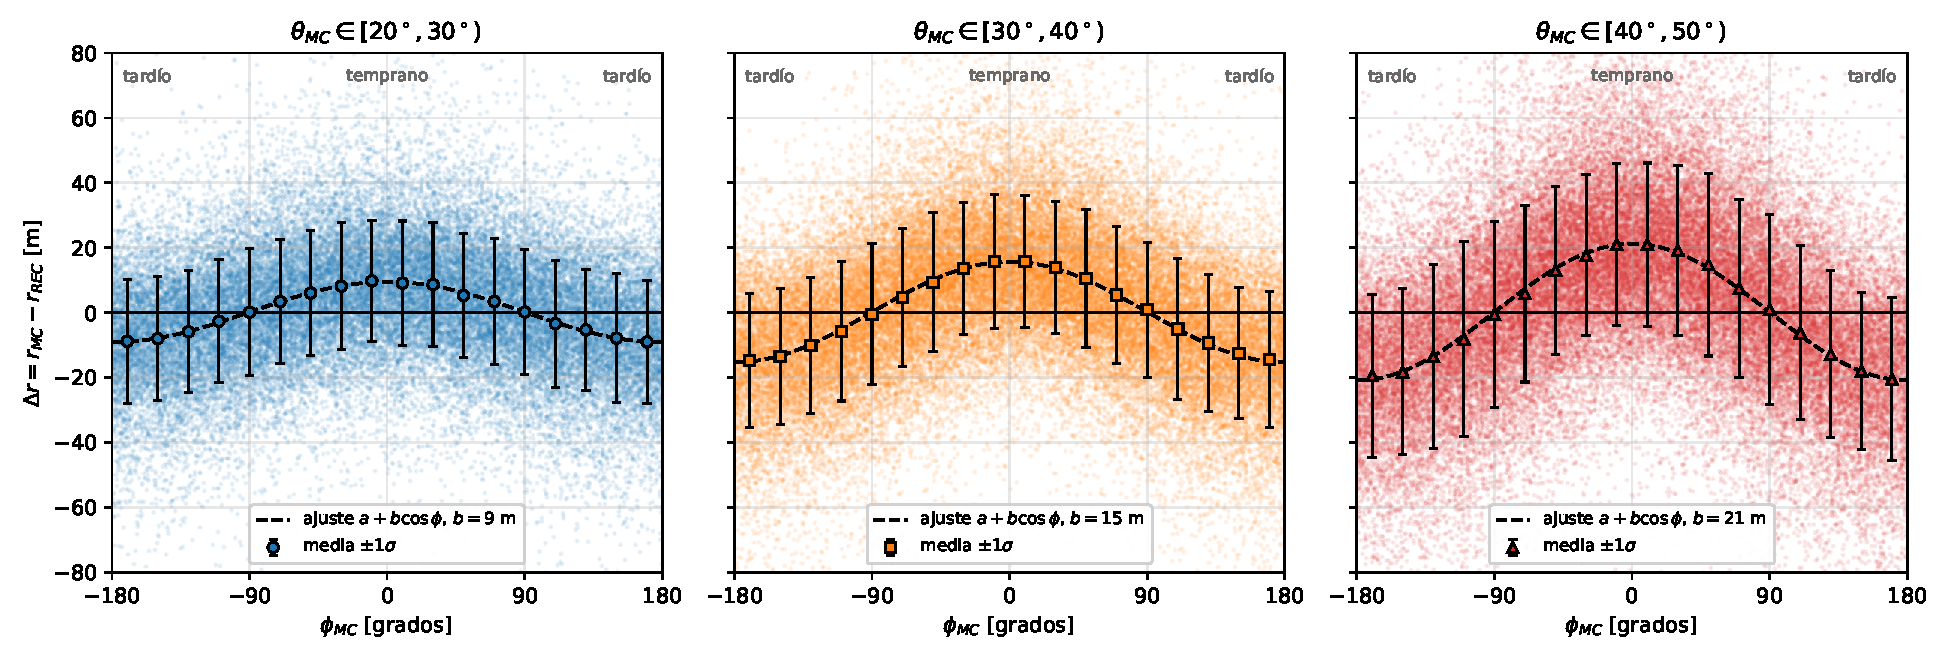
\includegraphics[width=0.7\linewidth]{tesis/corrimiento_nucleo_azimut.pdf}\\[0pt]
  \begin{columns}[T,onlytextwidth]
    \column{0.42\textwidth}
      \small
      Una función lateral \textbf{simétrica} ajustada a una señal
      \textbf{asimétrica} acerca el núcleo al exceso temprano ($b\simeq9$, 15,
      21\,m). Con $\rho\propto r^{-\beta}$: \;$\Delta A_1\simeq-\beta\,b/r$.
    \column{0.55\textwidth}
      {\scriptsize
      \begin{tabular}{@{}lcccc@{}}
        \toprule
        $\theta$ & $A_1$ (MC) & $A_1$ (REC) & $\Delta A_1$ obs. & $-\beta b/r$ \\
        \midrule
        20--30$^\circ$ & 0,062 & 0,011 & $-0{,}051$ & $-0{,}051$ \\
        30--40$^\circ$ & 0,086 & 0,002 & $-0{,}084$ & $-0{,}081$ \\
        40--50$^\circ$ & 0,108 & $-0{,}002$ & $-0{,}110$ & $-0{,}102$ \\
        \bottomrule
      \end{tabular}}\\[3pt]
      {\footnotesize 450--600\,m. La \textbf{distancia} explica casi toda la
      pérdida: un sesgo \textbf{estimable}, no ruido.}
  \end{columns}
  \creditoizq{Figura y tabla: tesis, Cap.~5 y 6. Núcleo verdadero menos reconstruido, en función del azimut}
\end{frame}

% ---------------------------------------------------------------- 39
\begin{frame}{Primera mirada a los datos de campo}
  \begin{columns}[c,onlytextwidth]
    \column{0.56\textwidth}
      \centering
      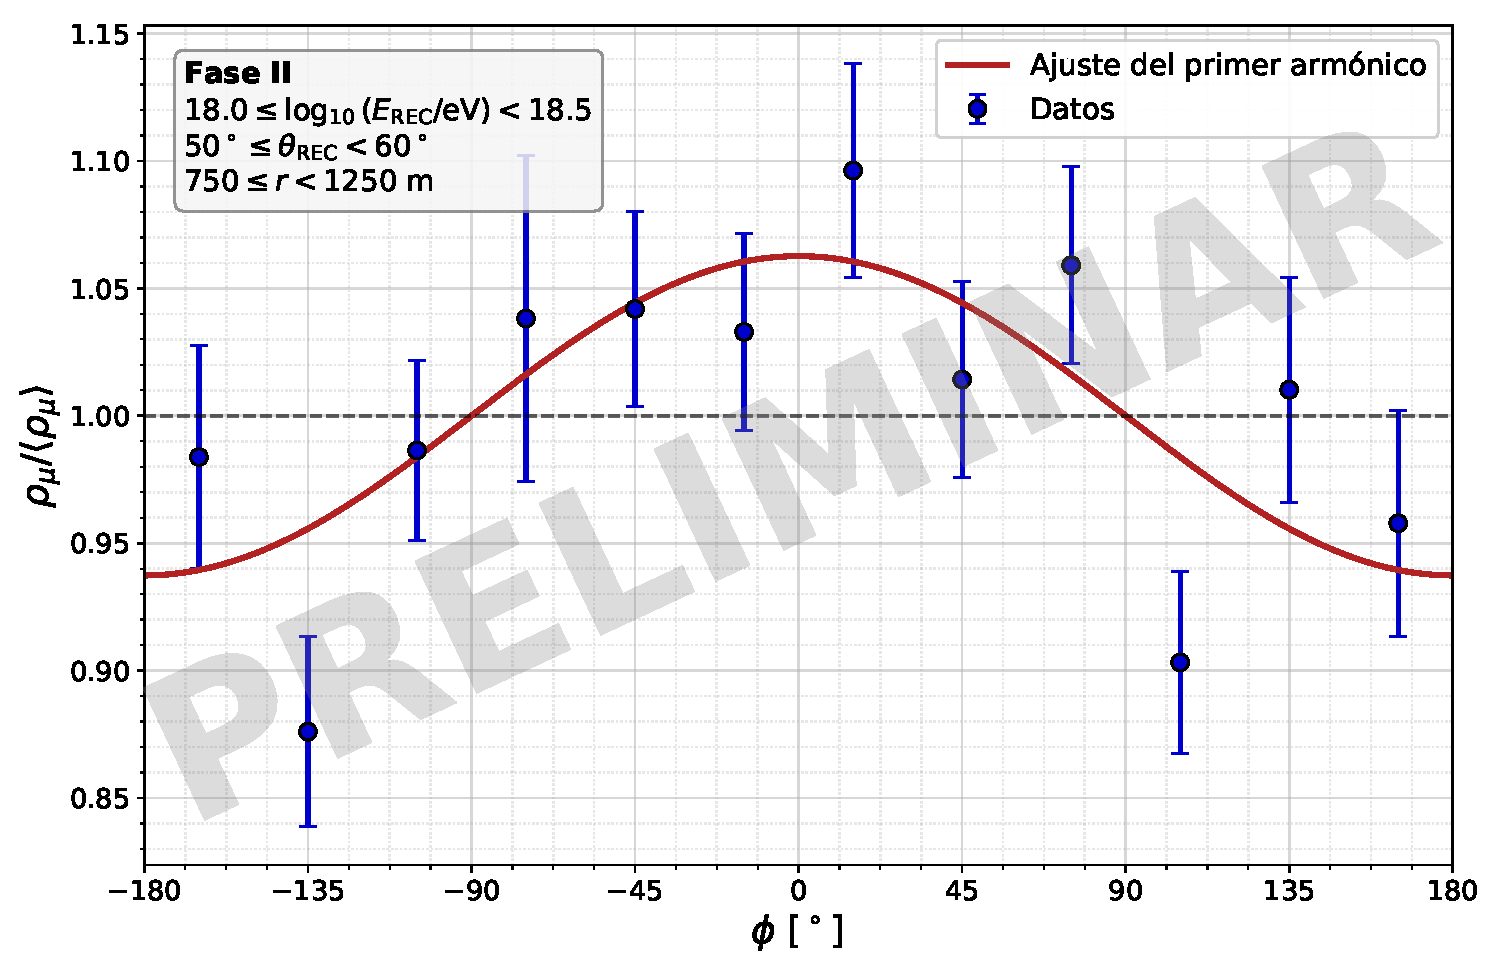
\includegraphics[width=\linewidth]{tesis/datos_campo_preliminar.pdf}
    \column{0.41\textwidth}
      \small
      UMD, arreglo de 750\,m, Fase II.\\
      {\footnotesize $18{,}0\le\lg(E/\mathrm{eV})<18{,}5$, \;$50^\circ\le\theta<60^\circ$,
      \;$750\le r<1250$\,m}
      \[ A_1 = 0{,}063\pm0{,}017 \]
      {\footnotesize Máximo en la región temprana, como predicen las
      simulaciones. Faltan los sistemáticos.}\\[4pt]
      \begin{clave}
        Hasta donde sabemos, la primera observación de esta asimetría con
        \textbf{muones aislados} de la componente electromagnética.
      \end{clave}

  \end{columns}
  \begin{tikzpicture}[remember picture, overlay]
    \node[anchor=north east] at ([xshift=-0.3cm, yshift=-1.1cm]current page.north east) {\preliminar};
  \end{tikzpicture}
  \credito{Datos de la Colaboración Pierre Auger; análisis propio (tesis, Cap.~6). Resultado preliminar, no oficial.}
\end{frame}

% ---------------------------------------------------------------- 40
\begin{frame}{Desde Argentina, a la región y al mundo}
  \begin{columns}[c,onlytextwidth]
    \column{0.36\textwidth}
      \centering
      \begin{tikzpicture}
        \mapaSA{6.4cm}
        \tikzset{lugar/.style={fill=itedaOrange, draw=white, line width=0.9pt},
          rot/.style={font=\scriptsize\bfseries, text=white, fill=noche,
            fill opacity=0.7, text opacity=1, inner sep=1.2pt, rounded corners=1pt}}
        \filldraw[lugar] \geoSA{-58.4}{-34.6} circle (2.6pt);
        \node[rot, anchor=west] at \geoSA{-57.5}{-35.3} {Buenos Aires};
        \filldraw[lugar] \geoSA{-69.6}{-35.5} circle (2.6pt);
        \node[rot, anchor=east] at \geoSA{-70.6}{-36.0} {Malargüe};
        \filldraw[lugar] \geoSA{-65.8}{-28.5} circle (2.6pt);
        \node[rot, anchor=east] at \geoSA{-67.0}{-28.2} {Catamarca};
        \filldraw[lugar] \geoSA{-46.6}{-23.5} circle (2.6pt);
        \node[rot, anchor=west] at \geoSA{-45.5}{-24.2} {São Paulo};
        \filldraw[lugar] \geoSA{-35.2}{-5.8} circle (2.6pt);
        \node[rot, anchor=north] at \geoSA{-37.5}{-7.0} {Natal};
      \end{tikzpicture}
    \column{0.61\textwidth}
      \begin{tikzpicture}[x=1cm,y=0.82cm]
        \draw[itedaGray, thick] (0,0.3) -- (0,-5.4);
        \foreach \y/\f/\t in {
            0/{mar.\ 2026}/{\textbf{Reunión de la Colaboración Pierre Auger}: el encuentro de toda la colaboración, dos veces por año},
            -1.05/{jun.\ 2026}/{\textbf{SAMMA}: School on Astroparticle and Multi-messenger Astrophysics, ICTP-SAIFR, São Paulo},
            -2.1/{jul.\ 2026}/{\textbf{IDPASC School 2026}, Instituto Internacional de Física (UFRN), Natal},
            -3.15/{sep.\ 2026}/{\textbf{RAFA 2026}, Catamarca},
            -4.2/{nov.\ 2026}/{\textbf{Reunión de la Colaboración Pierre Auger}, presentando los resultados de la tesis}}{
          \fill[itedaOrange] (0,\y) circle (2.4pt);
          \node[font=\scriptsize\bfseries, anchor=east, text=itedaOrange] at (-0.15,\y) {\f};
          \node[font=\scriptsize, anchor=west, text width=7.6cm, align=left] at (0.15,\y) {\t};}
      \end{tikzpicture}\\[6pt]
      \begin{clave}
        Hacer física desde Argentina te conecta con la comunidad
        \textbf{latinoamericana} y con colaboraciones \textbf{internacionales}
        de cientos de investigadores.
      \end{clave}
      {\scriptsize\color{itedaGray} Tesis en ITeDA (2025--26), dirigida por
      J.\,M.~Figueira y F.~Sánchez; defensa en FCEN-UBA, octubre de 2026.}
  \end{columns}
  \creditoizq{Mapa: Natural Earth (dominio público)}
\end{frame}
